%=====================================================================
\section{A third problem -- real-time control of a stormwater pond}\label{sec:pond}
%=====================================================================

The third problem changes the time scale from days to hours and adds a
water-quality objective. A stormwater pond collects runoff from an
impervious catchment and releases it through a valve that can be opened or
closed every hour. The pond has two jobs that pull in opposite directions:
\begin{itemize}\itemsep1pt
\item \textbf{Peak-flow control:} keep the outflow downstream low. We
measure this with $Q_p$, the outflow exceeded only a fraction $p$ of the
time (the ``exceedance'' objective of OHQ, as in the St.~Francis
real-time-control study).
\item \textbf{Treatment:} hold water long enough for pollutants to settle
and degrade. We measure this with the \emph{young-water fraction} of the
outflow from OHQ's Laplace age tracer.
\end{itemize}
Holding water (valve nearly closed) makes it older, which is good for
treatment. But the pond is then full when the next storm arrives and it
overflows, which is bad for $Q_p$. Releasing keeps room but passes young,
untreated water. A good operator holds water in dry weather and makes room
before storms, which is a natural job for a forecast-aware learned policy.

\subsection{System and data}
\begin{figure}[h]
\centering
\resizebox{\textwidth}{!}{\begin{tikzpicture}[>=Stealth, font=\small]
  \draw[->, very thick, blue!60] (-4.2,1.6) node[above, font=\scriptsize, align=center]{hourly rain\\(NOAA, Beltsville MD)} -- (-4.2,0.8);
  \draw[thick, fill=gray!20] (-5.4,0.2) rectangle (-3.0,0.8);
  \node[font=\scriptsize] at (-4.2,0.5) {catchment 2 ha};
  \draw[->, very thick, blue!70] (-3.0,0.5) -- node[above, font=\scriptsize]{runoff} (-0.9,0.5);
  \fill[blue!15] (-0.6,-0.4) -- (-0.25,0.7) -- (2.25,0.7) -- (2.6,-0.4) -- cycle;
  \draw[thick] (-0.9,1.5) -- (-0.6,-0.4) -- (2.6,-0.4) -- (2.9,1.5);
  \draw[dashed] (-0.8,1.15) -- (2.8,1.15);
  \node[font=\scriptsize, above] at (1.0,1.15) {overflow crest, 2 m};
  \node at (1.0,0.1) {Pond};
  \draw[->, very thick, green!50!black] (2.7,-0.25) -- node[below, font=\scriptsize, align=center]{valve (underdrain)\\opening $u_t$ (agent)} (5.3,-0.25);
  \draw[->, thick, red!70] (2.9,1.25) -- node[above, font=\scriptsize]{overflow weir} (5.3,1.25);
  \node[draw, thick, fill=gray!10, minimum width=1.5cm, minimum height=2.1cm, align=center, font=\small] (cb) at (6.05,0.5) {catch\\basin};
  \draw[->, very thick, blue!70] (6.8,0.5) -- node[above, font=\scriptsize]{sewer pipe} node[below, font=\scriptsize, align=center]{measured:\\$Q(t)$, young load} (9.4,0.5);
  \node[draw, thick, fill=blue!5, minimum width=1.4cm, minimum height=1.0cm, align=center, font=\small] at (10.15,0.5) {fixed\\head};
\end{tikzpicture}}
\caption{The stormwater pond. Both the valve (underdrain) and the overflow
discharge into a catch basin, which drains to the receiving water (a fixed
head) through a sewer pipe. Flow and young-water load are measured on that
pipe.}
\label{fig:pond_schematic}
\end{figure}

\paragraph{Rainfall.} The pond is driven by observed rainfall from NOAA's
Hourly Precipitation Data network (HPD v2, NOAA NCEI): station USC00180700,
Beltsville, Maryland, which lies between Baltimore and Washington DC. The
record runs from 1948 to 2026 at hourly resolution. Values are converted from
hundredths of an inch to meters, and flagged or missing hours are kept as
gaps (\code{prepare\_rain.py}). Annual totals of 1{,}000--1{,}200~mm, and a
record 1{,}804~mm in 2018, match the regional climatology. Each episode is a
\textbf{three-year} window (26{,}280 hours), as in the St.~Francis study.
A short window lets a controller exploit end effects (see ``Closing
loopholes'' below), and $Q_p$ at a small $p$ needs a long record. No
three-year window is entirely complete, so windows may have at most 1\%
missing hours, which are taken as dry. Training windows start anywhere in
1980--2019 where this holds (in practice 1996--2017 starts, about 12
distinct years of weather). The test windows are the two disjoint periods
2020--2022 and 2023--2025, which the agent never sees. Because two windows
give weak statistics, the comparison is also made year by year (six test
years).

\paragraph{Catch basin.} Following the St.~Francis model, the valve and the
overflow weir both discharge into a \code{Catch basin} block (4~m$^2$,
\code{Sewer\_system.json}). It drains through a \code{Sewer\_pipe} (0.3~m
diameter, Manning $n=0.01$, 10\% slope; capacity about 34{,}000~m$^3$/d) to
a fixed head. Measuring at the pipe means that overflow water is counted
with the tracer concentration OHQ actually carries through the system.

\paragraph{Catchment and pond.} Runoff is the rain on a 2-ha impervious
catchment with runoff coefficient 0.9, entering the pond as a
piecewise-constant hourly inflow. The pond is OHQ's \code{Pond} block
(\code{Pond\_Plugin.json}), whose storage--depth relation is approximately
$S=\alpha h^\beta$, with $\alpha=250$, $\beta=2$. The overflow crest at
$h=2$~m corresponds to 1{,}000~m$^3$, about 55~mm of runoff from the
catchment. An overflow
weir (\code{wier}, $Q=440{,}000\,(h-2)^{1.5}$~m$^3$/d) discharges anything
above the crest.

\paragraph{The valve.} The valve is a new OHQ link type,
\code{controlled\_orifice} (added to \path{resources/Pond_Plugin.json}
during this work): the orifice law with the valve opening $u\in[0,1]$ as a
property,
\[
Q_{valve}=86400\,C_d\,u\,A_{max}\sqrt{2g}\;\frac{h}{\sqrt{h+\varepsilon}},
\qquad C_d=0.6,\ A_{max}=0.03~\text{m}^2,\ \varepsilon=1~\text{mm}.
\]
The factor $h/\sqrt{h+\varepsilon}$ equals $\sqrt h$ for any real head but
becomes linear near an empty pond. With the plain $\sqrt h$ law, whose
slope is infinite at $h=0$, the implicit solver failed whenever an open
valve drained the pond within an hour. The St.~Francis valve devices use
the same regularization. While checking this link against a hand
calculation, we found that OHQ currently evaluates a function of a
\emph{pure constant} as the constant itself: $\sqrt{19.6}$ written as
\code{\_sqr(19.6)} evaluated to 19.6, which made the valve 4.4$\times$ too
large. The link type therefore writes $\sqrt{2g}=4.427$ as a number, so that it
also works with library builds that predate the fix of that bug (since
committed to OHQ). Here $h$ is the head difference between the pond and the
catch basin.

\subsection{Measuring water age with the Laplace tracer}
OHQ's \code{AgeTracker\_laplace} constituent, set up exactly as in the
St.~Francis residence-time study (\code{add\_age.py}), carries a tracer at
concentration 1 in every inflow. The tracer decays at a first-order rate
$\lambda$ wherever it is. A parcel of water that has spent time $\tau$ in
the system therefore carries concentration $e^{-\lambda\tau}$. If the water
in the pond (or leaving it) is a mixture of parcels with age density
$p(\tau)$, its concentration is
\[
C=\int_0^\infty p(\tau)\,e^{-\lambda\tau}\,d\tau=\mathcal L\{p\}(\lambda),
\]
the Laplace transform of the age distribution evaluated at $s=\lambda$:
hence the name. With $\lambda=1$~d$^{-1}$, water younger than a few hours
counts almost fully ($e^{-\lambda\tau}\approx1$) and water older than a few
days hardly at all. So $C$ acts as a smooth ``fraction of young water'' with
a time scale of about one day. The \textbf{young-water fraction} of the
outflow over an episode is the exported tracer load divided by the outflow
volume:
\[
F_y=\frac{\int Q(t)\,C(t)\,dt}{\int Q(t)\,dt}.
\]

\subsection{OHQ model and checks}
The Python binding cannot create constituents or reactions, so each hour's
model is written as a small \code{.ohq} script and loaded with
\code{create\_from\_script}. The script holds the templates, the tracer and
its decay reaction, the pond (with the current storage and tracer
concentration as initial conditions), the valve with this hour's opening,
the weir and the outlet. It is solved with twelve 5-minute steps, again
single-threaded. The pipe's hourly volume and young-water load are taken
from the catch basin's balance: inflow from the pond (valve and weir fluxes
at the end-of-step pond state, the valve seeing the basin's water level)
minus the change in the basin's water and tracer content, minus tracer
decay in the basin. This is exact by construction, whereas integrating
OHQ's interpolated rate outputs left a 3\% balance error. The pipe-flow
samples from OHQ's output give the 5-minute flows used for $Q_p$. Checks:
\begin{itemize}\itemsep1pt
\item \textbf{Valve law:} the outflow implied by OHQ's storage drop over a
step matches the formula above, evaluated at the end-of-step depth
(backward Euler), to within 0.1\%.
\item \textbf{Tracer:} closed valve, $S_0=1{,}900$~m$^3$, $C_0=0.3$, inflow
2{,}000~m$^3$/d for one hour. A hand mass balance (tracer inflow $+83.3$,
decay $\lambda M\,\Delta t\approx-23.8$) gives $C\approx0.317$; OHQ gives
0.3168.
\item \textbf{Water balance} over 800-hour test runs closes to within
0.01~m$^3$ out of 1{,}400--3{,}100~m$^3$ of inflow.
\end{itemize}
\paragraph{Making it fast enough.} A typical hourly step costs 20--50~ms:
about 23~ms to parse the script and templates, plus the solve. Three
problems had to be fixed first:
\begin{enumerate}\itemsep1pt
\item \textbf{Inflow file.} OHQ re-reads the inflow time series at every
build. A whole-episode file (52{,}000 points for three years) made each
step take seconds, so each step now gets a two-point file for its own hour.
\item \textbf{Round-off states.} When the pond or catch basin empties,
storages of $10^{-7}$--$10^{-11}$~m$^3$ and decayed tracer concentrations
of $10^{-150}$ made OHQ's Newton iterations crawl, at 1--2~s per hour.
Values below 0.1~m$^3$ (pond) and 0.01~m$^3$ (basin) are therefore set to
exactly zero between steps.
\item \textbf{Lockstep rollouts.} Even then about 0.6\% of hours take
around a second. With 16 simulators advanced in lockstep, every step
waited for the slowest, and throughput collapsed to about 20 steps/s. The
trainer now lets each worker collect its rollout independently
(Section~\ref{sec:ppo}).
\end{enumerate}
At 20--50~ms per step, a three-year episode costs about 15--20 minutes of
CPU, the clearest case so far for a compiled (codegen) backend.

\subsection{Objectives, reward and the exceedance problem}
\paragraph{Evaluation metrics.} For each test window we compute, from the
outflow at every 5-minute solver step:
\begin{itemize}\itemsep1pt
\item $Q_p$ with $p=0.001$: the flow exceeded 0.1\% of the time (about 43
minutes per month), the value used in the St.~Francis study;
\item the young-water fraction $F_y$;
\item a scalar objective used to tune baselines and rank policies, with
each metric normalized by the \emph{passive} pond (valve fully open) under
the same rain:
\[
J=\frac{Q_p}{Q_p^{\,passive}}+\frac{F_y}{F_y^{\,passive}} .
\]
Lower is better. The passive pond scores exactly 2, and halving either
metric relative to doing nothing is worth the same. The normalization is
done per test window and per test year. For the tuning grid it uses the
passive pond's averages over the two tuning windows. Because any weighting
is a judgment call, we also show the full trade-off between $Q_p$ and
$F_y$.
\end{itemize}

\paragraph{Closing loopholes.} Earlier versions of this problem show how
readily an optimizer exploits gaps in an objective:
\begin{itemize}\itemsep1pt
\item With a pond twice as large (2{,}000~m$^3$) and 30-day episodes, the
best tuned rule kept the valve shut all month. A month's runoff fit in the
pond, so almost nothing left and $Q_p$ was near zero, and every window
ended with a full pond, a cost the window never saw. A realistically sized
pond (1{,}000~m$^3$) and three-year episodes remove this.
\item Water still in the pond or catch basin at the end of an episode is
counted as exported at its current tracer concentration, so holding water
to the end cannot hide young water.
\item With 30-day episodes, PPO learned to keep the pond near the crest and
let it overflow in short bursts. In the first model the overflow went
straight to the outlet and the age tracer treated it as old pond water.
Routing both the valve and the overflow through the catch basin, and
measuring there, makes OHQ carry the overflow's age consistently.
\end{itemize}
Following the design intent, there is no explicit penalty on overflow and
no minimum-storage rule. Overflow matters only through its effect on the
exceedance flow and on the young-water fraction, and the agent is free to
use it whenever that helps.

\paragraph{Choosing $p$.} We first used $p=0.01$. Over a 30-day window that
is about 7 hours, and a short overflow lasting less than that falls entirely
inside the ignored 1\%. A rule that kept the valve shut and let the pond
overflow scored a $Q_p$ of only 264~m$^3$/d despite overflow peaks of
8{,}800~m$^3$/d. With $p=0.001$, $Q_p$ reflects such peaks, and the training
surrogate (which penalizes every high flow) and the evaluation metric agree.

\paragraph{Why not use $Q_p$ as the reward directly?} RL maximizes a
\emph{sum} of per-step rewards (Section~\ref{sec:primer_math}). A quantile
is not a sum: whether a particular hour's flow matters depends on all other
hours of the episode. Its only exact form would be a single reward at the
very end of the 720-hour episode, which gives the agent almost no signal
about which hours mattered. We therefore train on a smooth
\emph{surrogate} that is additive, and evaluate on the exact $Q_p$:
\[
r_t=-w_q\,\frac{1}{\Delta t}\sum_{n}\Big(\frac{\max(0,\,Q_n-Q_{ref})}{Q_{ref}}\Big)^2\delta t
\;-\;w_y\,\frac{\sum_n Q_n C_n\,\delta t}{V_{ref}},
\]
summed over the solver steps $n$ of hour $t$. The first term penalizes
flows above $Q_{ref}$, and penalizes large ones much more because of the
square, which pushes down the upper tail of the flow distribution, where
$Q_p$ lives. The second term is the exported young-water load, which is
additive, so it represents $F_y$ exactly up to the (nearly policy-independent)
total outflow volume. Here $w_q=1$, $w_y=5$ and $V_{ref}=1{,}000$~m$^3$. The
weights roughly mirror $J$: with $Q_p^{\,passive}\approx5{,}000$~m$^3$/d and
$F_y^{\,passive}\approx1$, $J\propto Q_p/1{,}000+5F_y$.

\paragraph{Observation and action.} The agent observes 9 numbers: pond
depth, pond tracer concentration $C$, current inflow, noisy rain forecasts
for the next 1, 3, 6, 12 and 24 hours (multiplicative log-normal error
growing with lead time), and the fraction of the window left. It sets the
valve opening once per hour. The network's action $a_t\in[-1,1]$ is mapped
to the opening as $u_t=((a_t+1)/2)^2$. With the linear mapping used at
first, the useful openings of 0--10\% occupied only the bottom 5\% of the
action range; with the square they occupy about a third of it.

\subsection{Baselines}
\begin{itemize}\itemsep1pt
\item \textbf{Open valve} ($u=1$): a conventional dry pond with a fixed
orifice.
\item \textbf{Fixed opening} $u$: a throttled orifice; $u$ tuned over $\{0.03,0.05,0.1,0.2,1\}$.
\item \textbf{Forecast rule}, in the spirit of the St.~Francis
forecast-informed control: hold at a small opening $u_{hold}$ so that water
ages; when the 24-hour rain forecast exceeds a threshold, pre-release at
$u_{pre}$; open fully if the depth exceeds 1.8~m. The three parameters are
tuned by grid search over 24 combinations ($u_{hold}\in\{0,0.02\}$, $u_{pre}\in\{0.05,0.1,0.2,0.4\}$, threshold $\in\{10,15,30\}$~mm), centred on the best settings found with 30-day windows.
\end{itemize}
Both rule families are tuned on two three-year training-period windows
(starting 1996 and 2009); the results are fixed opening $u=0.02$; forecast rule $u_{hold}=0$, $u_{pre}=0.1$, threshold 15~mm.

\begin{figure}[h]
\centering
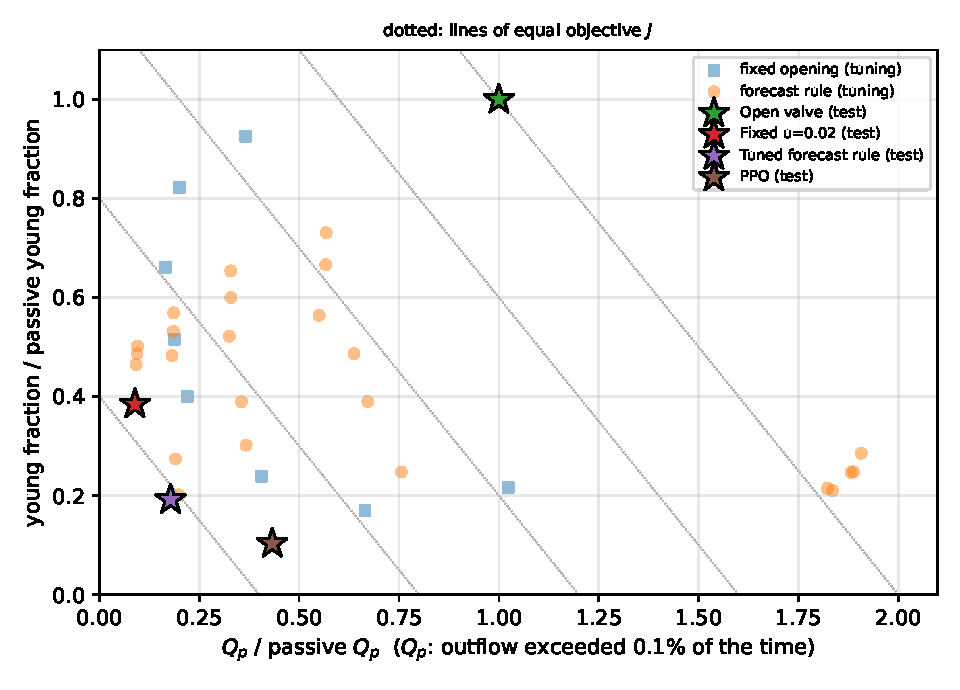
\includegraphics[width=0.7\textwidth]{figures/pond_tradeoff.pdf}
\caption{Trade-off between peak-flow control ($Q_p$) and treatment (young
fraction). Small symbols: every baseline setting tried during tuning
(training windows). Stars: the four compared policies on the test windows.
Dotted lines connect points with equal objective $J$.}
\label{fig:pond_tradeoff}
\end{figure}

\subsection{Training}
The first attempt trained PPO from scratch with a linear action mapping and
raw rewards. It converged to a poor policy that opened the valve only when
the pond was already empty, kept the pond at the crest, and scored a
normalized $J$ of 1.13--1.23 on the test windows, barely better than the
passive pond's 2. The run evaluated in Tables~\ref{tab:pond_results} and~\ref{tab:pond_paired}
uses the three remedies described in
Section~\ref{sec:ppo}: the square action mapping, reward normalization, and
a warm start by behavior cloning of the tuned forecast rule. The cloned
actor reproduced the rule's 48{,}000 decisions to within 0.008 on the action
scale. PPO then trained for 1.5 million hourly steps, about 2.5 hours on a
machine shared with other jobs. Its first rollouts already scored at the
rule's level (about $-0.005$ per hour, versus $-0.10$ from scratch). The
raw reward per hour kept improving to about $-0.0004$ by the end, and the
exploration spread fell from 0.30 to 0.13. A second warm-started run without reward clipping, with snapshot selection by $J$, is
described at the end of the results.


\begin{figure}[h]
\centering
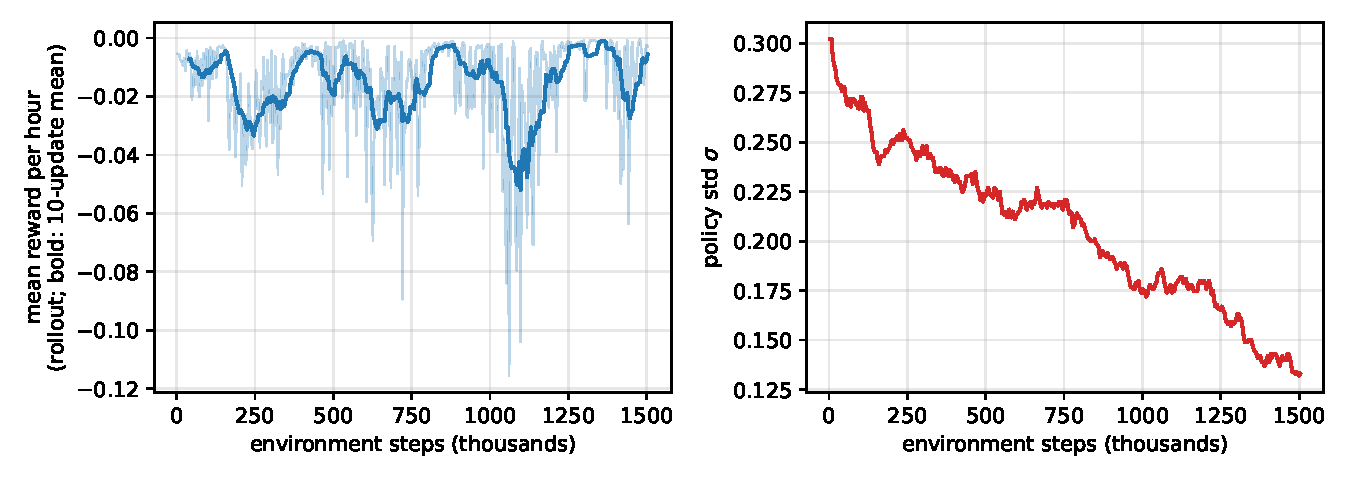
\includegraphics[width=0.95\textwidth]{figures/pond_learning_curve.pdf}
\caption{Pond training: mean return of the last 20 episodes (left), policy
standard deviation (right).}
\label{fig:pond_learning}
\end{figure}

\subsection{Results}
\begin{table}[h]
\centering
\small
\begin{tabular}{lrrrrrr}
\toprule
Policy & window & $J$ & $Q_p$ [m$^3$/d] & young fraction & peak [m$^3$/d] & overflow [m$^3$] \\
\midrule
Open valve & 2020--22 & 2.00 & 5182 & 0.993 & 8391 & 0 \\
 & 2023--25 & 2.00 & 4971 & 0.993 & 8558 & 0 \\
Fixed u=0.02 & 2020--22 & 0.50 & 697 & 0.361 & 11986 & 2349 \\
 & 2023--25 & 0.45 & 216 & 0.403 & 11525 & 1384 \\
Tuned forecast rule & 2020--22 & 0.37 & 912 & 0.197 & 12056 & 162 \\
 & 2023--25 & 0.36 & 896 & 0.183 & 11111 & 85 \\
PPO & 2020--22 & 0.59 & 2487 & 0.107 & 12309 & 11819 \\
 & 2023--25 & 0.48 & 1917 & 0.097 & 12195 & 6277 \\
\bottomrule
\end{tabular}

\caption{Pond: results for the two three-year test windows. $J$ is the
evaluation objective (lower is better).}
\label{tab:pond_results}
\end{table}

\begin{table}[h]
\centering
\small
\begin{tabular}{lrrrr}
\toprule
baseline & mean $\Delta J$ (per year) & std.\ error & PPO better in & mean $\Delta Q_p$ / $\Delta$young \\
\midrule
Open valve & $-1.494$ & 0.054 & 6/6 years & $-3031$ / $-0.892$ \\
Fixed u=0.02 & $+0.031$ & 0.050 & 2/6 years & $+1616$ / $-0.281$ \\
Tuned forecast rule & $-0.078$ & 0.216 & 2/6 years & $-12$ / $-0.088$ \\
\bottomrule
\end{tabular}

\caption{Pond: paired differences, PPO minus baseline, computed for each
of the six test years. Negative $\Delta J$ means PPO is better.}
\label{tab:pond_paired}
\end{table}

\paragraph{Headline.} Over the full three-year test windows, the tuned
forecast rule is the best policy ($J=0.375$ and 0.365, i.e.\ about 82\%
better than the passive pond). Next come the 2\% fixed opening (0.498,
0.450) and PPO (0.588, 0.483). Year by year, PPO and the rule are
statistically tied ($\Delta J=-0.08\pm0.22$, PPO better in 2 of 6 years).
The three-year metric, the St.~Francis definition, favors the rule because
PPO's overflows cluster in a few years and raise the three-year $Q_p$.
The warm start made a large difference: from scratch, PPO scored
$J\approx1.1$--1.2.

\paragraph{What PPO changed relative to the rule.} PPO started as an exact
copy of the rule and moved toward holding more water. Its outflow is the
oldest of all policies (young fraction 0.10--0.11, versus 0.18--0.20 for
the rule). But it ends both windows at the crest and overflows
6{,}000--12{,}000~m$^3$ per window (the rule: 85--162~m$^3$). Its $Q_p$ is
therefore 2--3 times the rule's. In terms of $J$, the gain in age does not
pay for the loss in peak-flow control.

\paragraph{Why: the training reward is not exactly $J$.} During training
PPO kept improving the reward it was given: the raw reward per hour
improved from $-0.028$ to $-0.0004$. That reward differs from $J$ in two
ways, and both undervalue overflow:
\begin{enumerate}\itemsep1pt
\item the peak term is a smooth surrogate of the exceedance quantile, not
the quantile itself;
\item reward normalization \emph{clips} rewards at $\pm10$ standard
deviations. That stabilized learning, but it also caps the penalty of
exactly the rare, extreme overflow hours that determine $Q_p$.
\end{enumerate}
So PPO optimized the stated reward well, but the stated reward traded
overflow for age at a different rate than $J$ does.

\paragraph{What would likely close the gap.}
\begin{itemize}\itemsep1pt
\item Normalize rewards without clipping (or with a much wider clip), so
the overflow penalty keeps its weight.
\item Select the policy by $J$: evaluate checkpoints during training on
held-out training-period windows and keep the best one, rather than the
last.
\item Keep the policy close to the rule unless it clearly improves on it,
e.g.\ by penalizing deviation from the cloned rule early in training.
\end{itemize}

\paragraph{Lessons.} Two lessons stand out. First, starting from an
engineering rule turned an RL failure into a policy competitive with a
carefully tuned rule. Second, when the true objective (a quantile over
three years) cannot be the reward, every simplification of it, including
the numerical stabilizations, becomes part of the objective the agent
actually optimizes. Whether the result is better must be judged on the
true objective, with tuned baselines, on data the agent has not seen.


\begin{figure}[h]
\centering
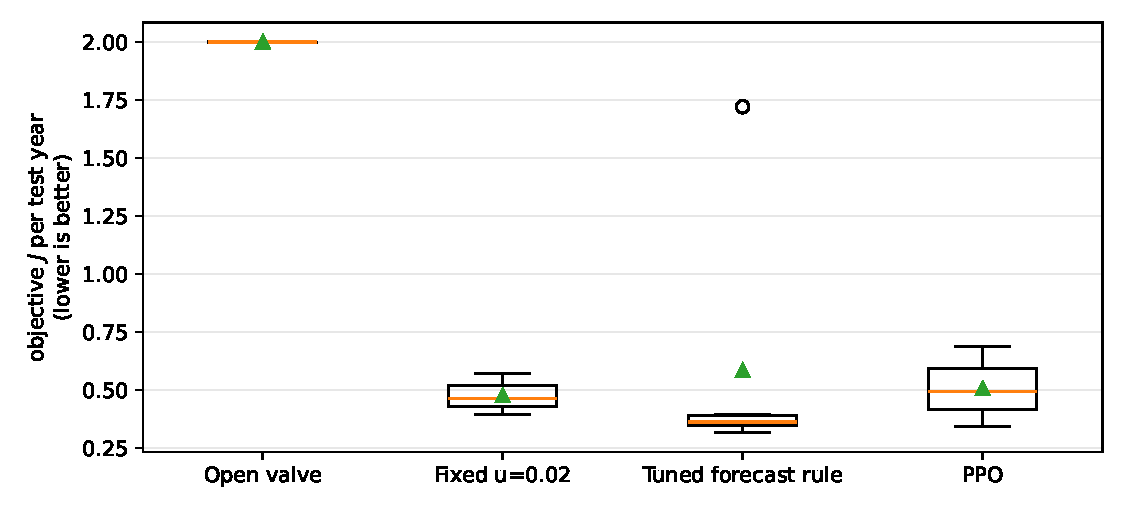
\includegraphics[width=0.7\textwidth]{figures/pond_J_boxplot.pdf}
\caption{Pond: distribution of the objective $J$ over the six test years.}
\end{figure}

\begin{figure}[p]
\centering
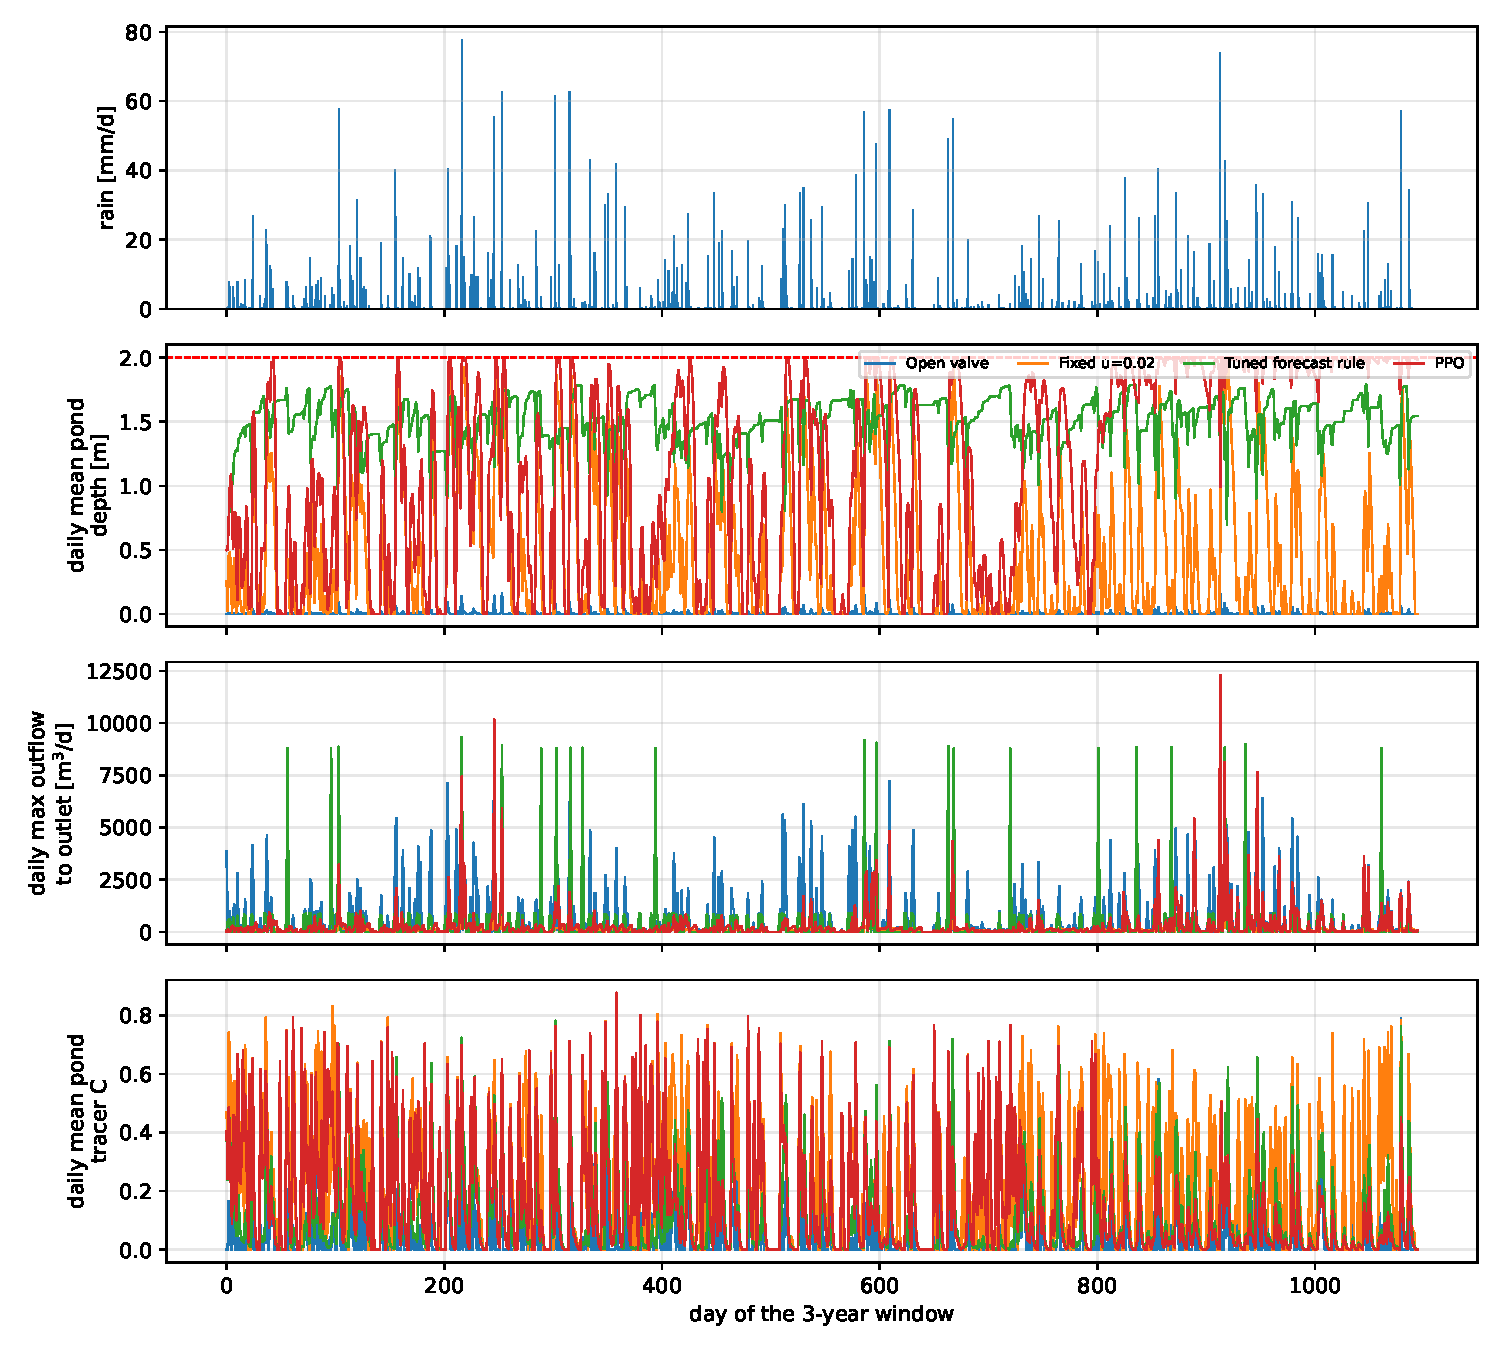
\includegraphics[width=0.92\textwidth]{figures/pond_trajectory_window0.pdf}
\caption{Test window 2020--2022, daily values. From top: daily rain; daily
mean pond depth (dashed: overflow crest); daily maximum flow to the outlet;
daily mean pond tracer concentration (lower means older water).}
\label{fig:pond_traj_w0}
\end{figure}

\begin{figure}[p]
\centering
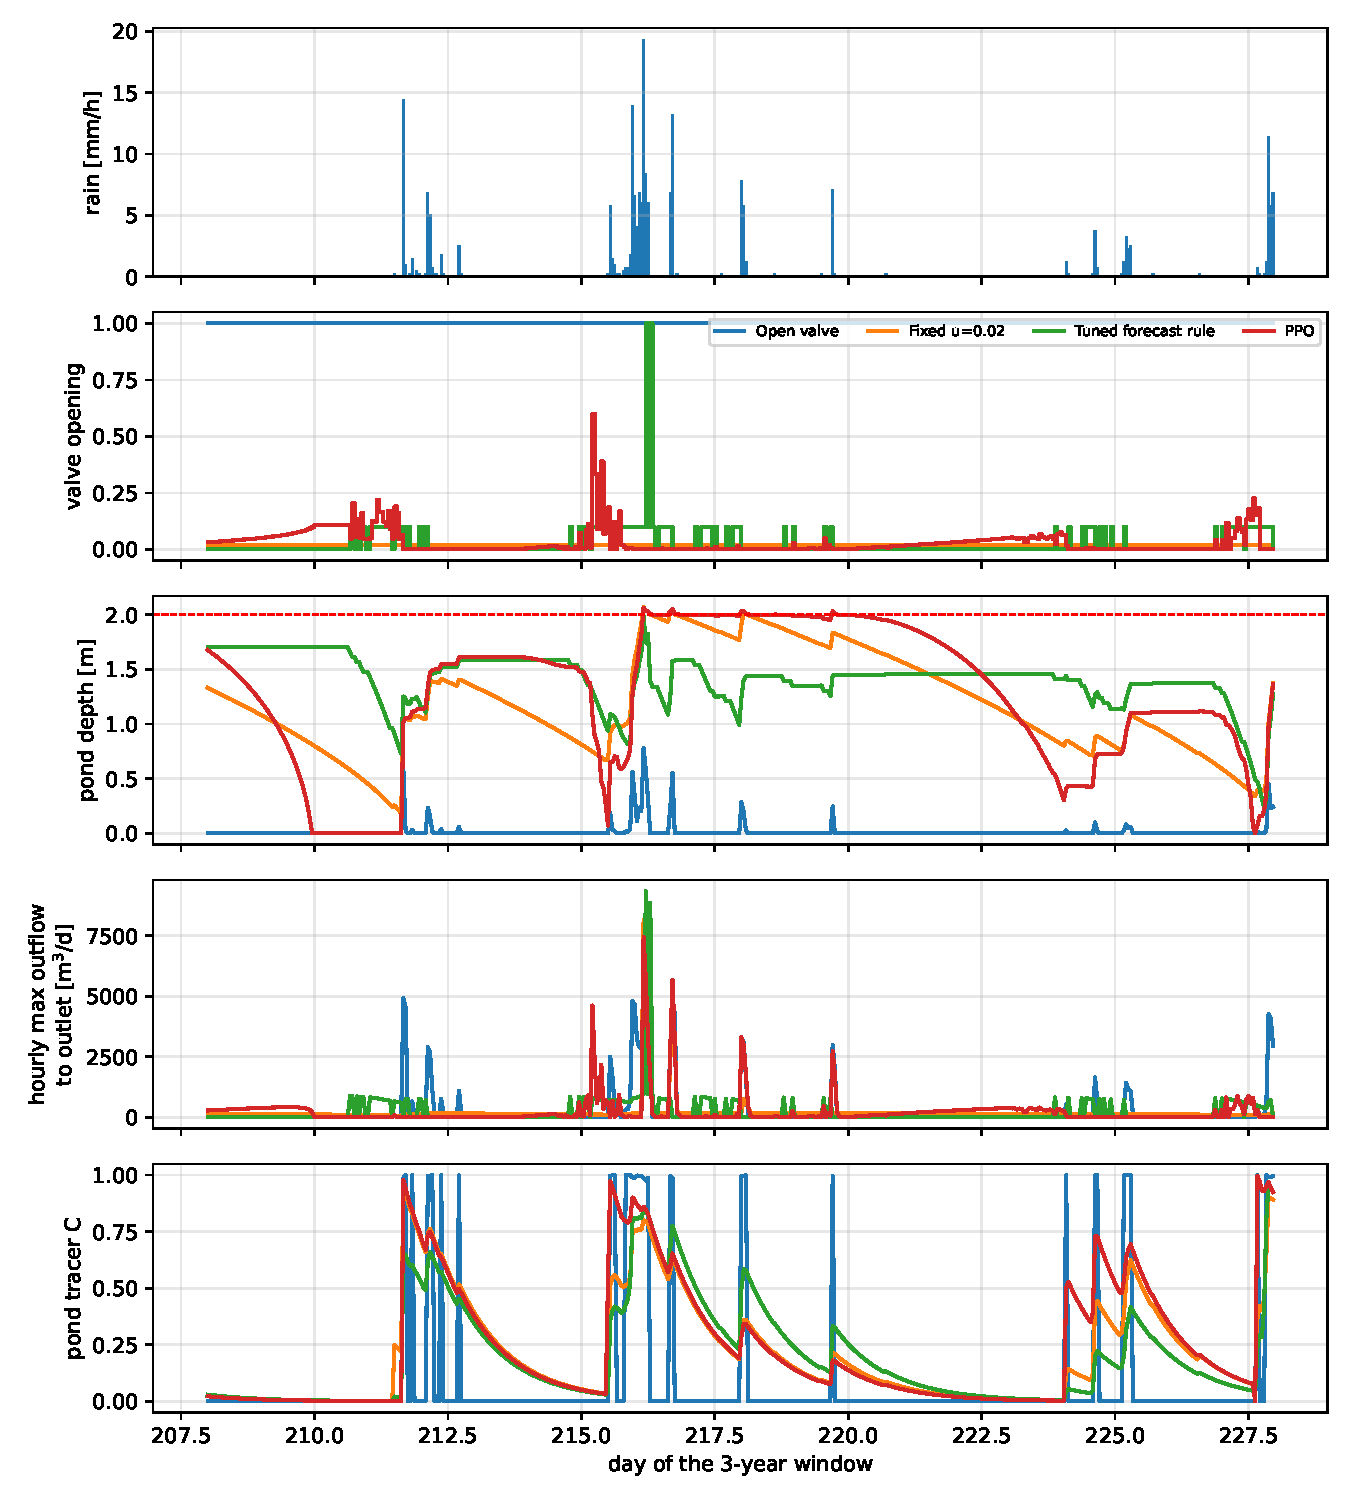
\includegraphics[width=0.92\textwidth]{figures/pond_trajectory_window0_zoom.pdf}
\caption{Test window 2020--2022, hourly detail of the 20 days around the
wettest day. From top: rain; valve opening; pond depth; hourly maximum flow
to the outlet; pond tracer concentration.}
\label{fig:pond_traj_w0_zoom}
\end{figure}

\begin{figure}[p]
\centering
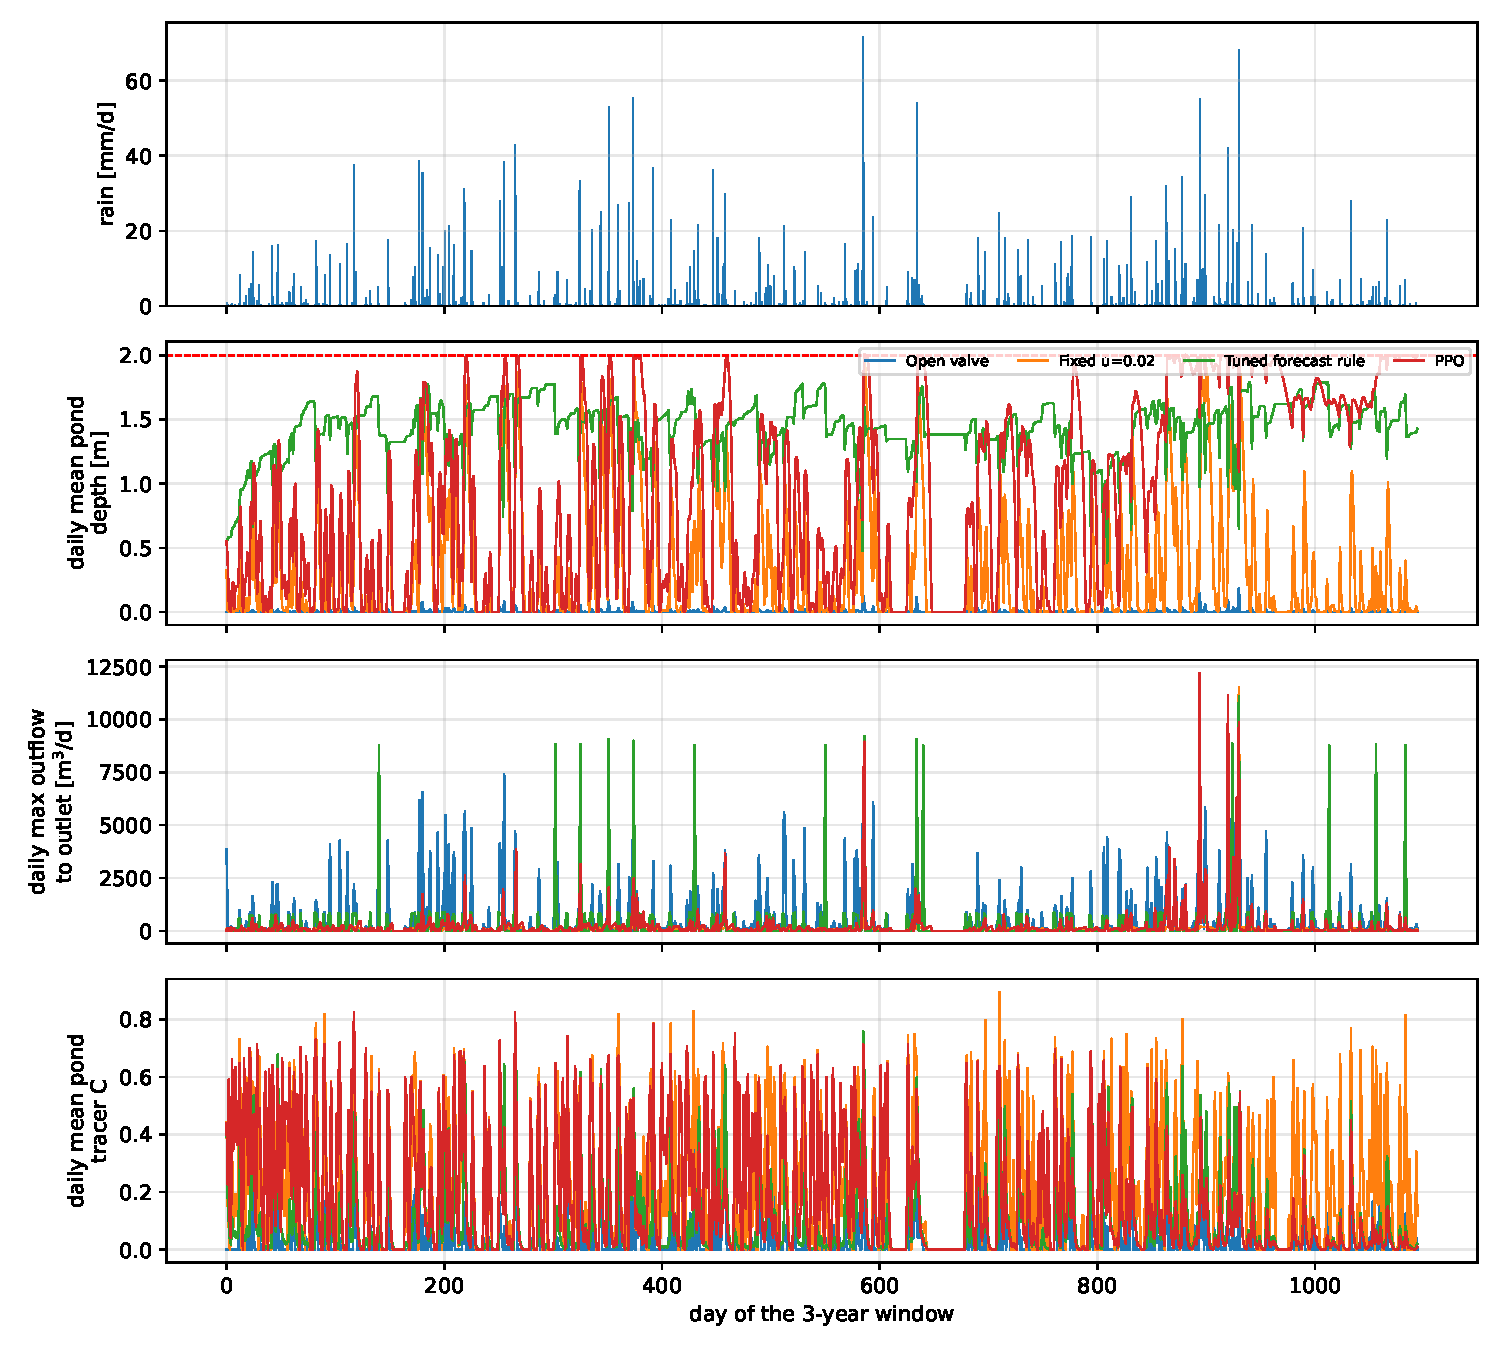
\includegraphics[width=0.92\textwidth]{figures/pond_trajectory_window1.pdf}
\caption{Test window 2023--2025, daily values (panels as in Figure~\ref{fig:pond_traj_w0}).}
\label{fig:pond_traj_w1}
\end{figure}

\begin{figure}[p]
\centering
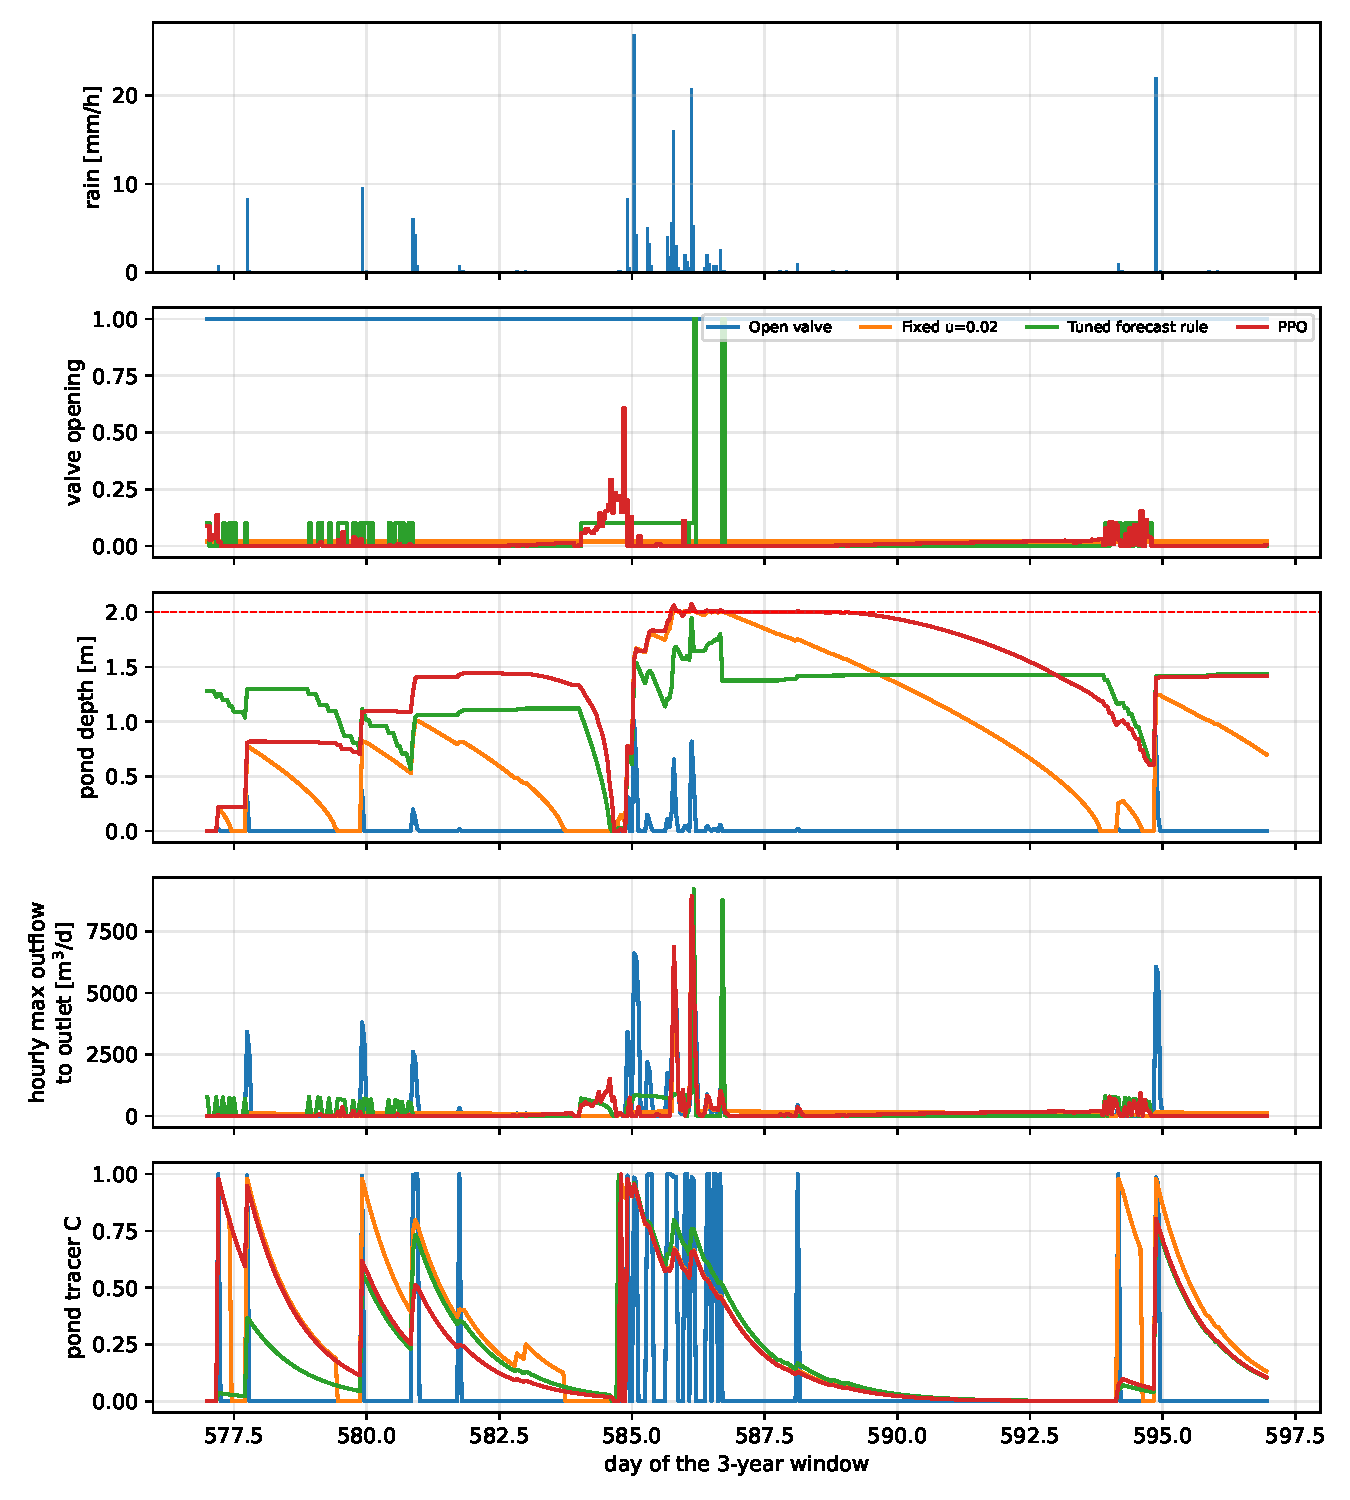
\includegraphics[width=0.92\textwidth]{figures/pond_trajectory_window1_zoom.pdf}
\caption{Test window 2023--2025, hourly detail around the wettest day.}
\label{fig:pond_traj_w1_zoom}
\end{figure}
